\documentclass{article}
\usepackage{import}
\import{../../lib/latex/}{wgmlgz}


\begin{document}

\itmo[
      variant=666666666,
      labn=2,
      discipline=Основы профессиональной деятельности,
      group=P3115,
      student=Владимир Мацюк,
      teacher=Пашнин Александр Денисович
]
\lstset{language=Python}

\tableofcontents

\section{Задание}
По выданному преподавателем варианту определить функцию, вычисляемую программой, область представления и область допустимых значений исходных данных и результата, выполнить трассировку программы, предложить вариант с меньшим числом команд. При выполнении работы представлять результат и все операнды арифметических операций знаковыми числами, а логических операций набором из шестнадцати логических значений.
\begin{center}
      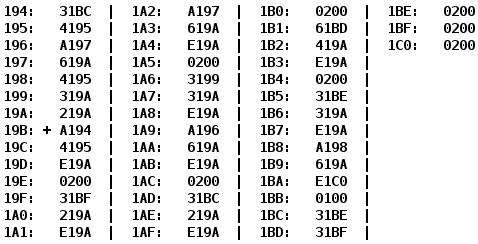
\includegraphics[scale=0.5]{task.png}
\end{center}

\begin{tabular}{|c|r|l|l|} \hline
      Адрес & Код команды & Мнемоника & Комментарии \nl
      178   & E184        & ST 184    & \nl
      179   & 0100        & HLT       & \nl
      17A   & 0200        & CLA       & \nl
      17B   & + 0200      & CLA       & \nl
      17C   & 6178        & SUB 178   & \nl
      17D   & 6179        & SUB 179   & \nl
      17E   & E183        & ST 183    & \nl
      17F   & A17A        & LD 17A    & \nl
      180   & 2183        & AND 183   & \nl
      181   & E184        & ST 184    & \nl
      182   & 0100        & HLT       & \nl
      183   & 2183        & AND 183   & \nl
      184   & 2183        & AND 183   & \nl
\end{tabular}
\section{Вывод}
Я познакомился с форматами файлов JSON, XML и написал парсер JSON на Python .
\end{document}
